% $ platex body
% $ dvipdfmx body

\documentclass[a4j]{jarticle}

\title{「データ解析入門」レポート}
\author{1677281 山内 拓弥}
\usepackage{colortbl}
\usepackage[dvipdfmx]{graphicx}
\renewcommand{\thesection}{課題\arabic{section}}
\renewcommand{\thesubsection}{}

\begin{document}

\maketitle

\section{}
クラスタリングとベクトル量子化の定義を、
その違いがわかるように説明し、
平方和最小基準クラスタリング問題と2乗誤差に基づくベクトル量しか問題の
局所最適解における性質について記述しなさい。

\subsection{【回答】}
TBD

\section{}
教科書の「HokkaidoTowns\_xy\@.dat」データを、 k-meansアルゴリズムと競合学習で、
6分割にクラスタリングする実験を行い、 その結果を示し、考察しなさい。
具体的には、プログラムに与える引数である「乱数の種」、
「学習率」(競合学習のみ)などをいくつか変更して実験を行い、
両手法の性能比較を行いなさい。

\subsection{【回答】}

\paragraph{[乱数の種を振り、k-meansアルゴリズムと競合学習を比較]}
本実験では、2乗誤差の$E_Q$と$J_W$の傾向を、
k-meansアルゴリズムと競合学習とで比較した。
k-meansアルゴリズム、競合学習ともに、乱数を変えながら10回試行した。
競合学習の学習率は0.001とした。
結果を表\ref{tab:k-mean-comp}に示す。
競合学習の結果は安定している一方、
k-meansアルゴリズムは、表\ref{tab:k-mean-comp}のグレーのセルに示すように、
悪い結果が出ることがある。

\begin{table}[tbp]
 \begin{center}
  \caption{k-meansアルゴリズム、競合学習、2乗誤差比較}
  \label{tab:k-mean-comp}
  \begin{tabular}{|r||r|r|r|} \hline
            & k-means     & \multicolumn{2}{|c|}{競合学習} \\ \cline{2-4}
   試行番号 & $E_Q = J_W$                  & $E_Q$  & $J_W$  \\ \hline \hline
          1 &                       474825 & 472490 & 472288 \\ \hline
          2 & \cellcolor[gray]{0.8} 543956 & 472673 & 472217 \\ \hline
          3 &                       474825 & 472577 & 472288 \\ \hline
          4 & \cellcolor[gray]{0.8} 609216 & 472959 & 472808 \\ \hline
          5 &                       473367 & 472557 & 472288 \\ \hline
          6 &                       473367 & 472501 & 472288 \\ \hline
          7 &                       472288 & 472439 & 472217 \\ \hline
          8 & \cellcolor[gray]{0.8} 503663 & 472648 & 472288 \\ \hline
          9 &                       472769 & 472429 & 472288 \\ \hline
         10 &                       474818 & 472367 & 472217 \\ \hline
  \end{tabular}
 \end{center}
\end{table}

k-meansアルゴリズムの悪い結果は、
局所最適解になっていると考えられる。
良い結果の一例として試行番号1
のクラスタリング結果を図\ref{fig:Hokkaido_xyl_seed1}に示す。
また、悪い結果の一例として試行番号4
のクラスタリング結果を図\ref{fig:Hokkaido_xyl_seed4}に示す。
これらの間には、
\begin{itemize}
\item 図\ref{fig:Hokkaido_xyl_seed4}ではCluster3と4が広い。
\item 図\ref{fig:Hokkaido_xyl_seed1}のCluster5に相当する地域は、
      図\ref{fig:Hokkaido_xyl_seed4}ではCluster2と5に分割されている。
\end{itemize}
といった差異が見られる。
また、競合学習のクラスタリング結果を図\ref{fig:Hokkaido_xyl_compLearn}
に示す。k-meansアルゴリズムの良い結果である図\ref{fig:Hokkaido_xyl_seed1}
と似ていることがわかる。

\begin{figure}[tbp]
 \begin{minipage}{0.5\hsize}
  \begin{center}
   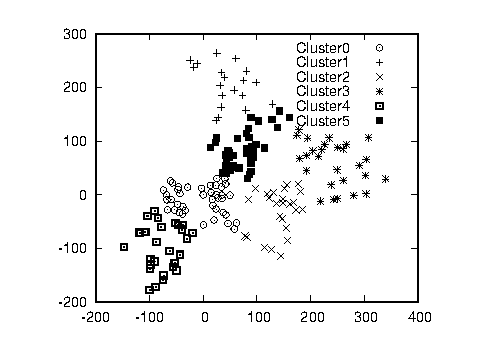
\includegraphics[width=\hsize]{fig/Hokkaido_xyl_seed1.eps}
  \end{center}
  \caption{k-meanアルゴリズム、良い結果}
  \label{fig:Hokkaido_xyl_seed1}
 \end{minipage}
 \begin{minipage}{0.5\hsize}
  \begin{center}
   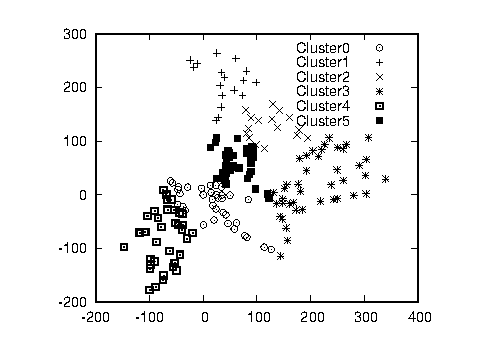
\includegraphics[width=\hsize]{fig/Hokkaido_xyl_seed4.eps}
  \end{center}
  \caption{k-meanアルゴリズム、悪い結果}
  \label{fig:Hokkaido_xyl_seed4}
 \end{minipage}
\end{figure}

\paragraph{競合学習の学習率と2乗誤差の関係}

学習率を振って、反復終了時の2乗誤差$E_Q$と$J_W$を調べた。
結果を図\ref{fig:compLearn}に示す。
横軸は学習率、縦軸は$E_Q$と$J_W$である。
学習率が$10^{-4}$から$10^{-2}$の範囲では、$E_Q$、$J_W$
共に$4.7\times 10^5$付近で安定している。
これより学習率が小さくても大きくても、反復終了時の$E_Q$、$J_W$は大きく、
すなわち悪くなる。
学習率が小さい時は、重みベクトルが収束し切らないため、
反復終了時の$E_Q$、$J_W$が大きくなっていると考えられる。
学習率が大きい時は、局所最適解の近傍まではたどり着くが、
1反復あたりの重みベクトルの変化量が大きく、
局所最適解からに近づき切れないため$E_Q$、$J_W$
が大きい値にとどまっていると考えられる。

\begin{figure}[tbp]
 \begin{minipage}{0.5\hsize}
  \begin{center}
   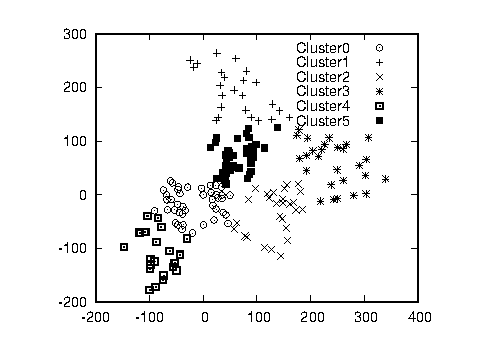
\includegraphics[width=\hsize]{fig/Hokkaido_xyl_compLearn.eps}
  \end{center}
  \caption{競合学習、学習率$=0.001$のクラスタリング結果}
  \label{fig:Hokkaido_xyl_compLearn}
 \end{minipage}
 \begin{minipage}{0.5\hsize}
  \begin{center}
   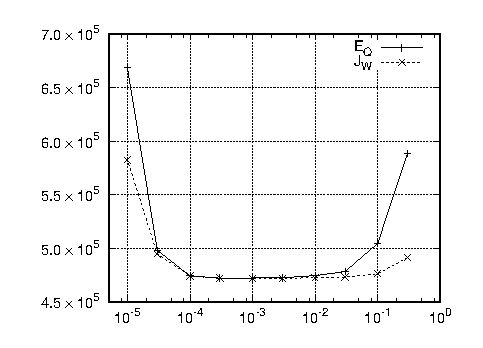
\includegraphics[width=\hsize]{fig/compLearn.eps}
  \end{center}
  \caption{競合学習、学習率と$E_Q$、$J_W$}
  \label{fig:compLearn}
 \end{minipage}
\end{figure}

\section{}
教科書の「HokkaidoTowns\_xy\@.dat」データを、
k-meansアルゴリズムなどで6分割したクラスタリングを行い、
その結果を「Hokkaido\_xyl\@.dat」としなさい。
次に、修正パーセプトロン学習プログラムであるmodPerceptronを用い、
上記クラスタリング結果を学習パターンとして学習させなさい。
その時、「乱数の種」、「学習率」を変化させて実験し、
収束するまでの繰り返し回数の傾向について考察しなさい。

\subsection{【回答】}
TBD

\begin{figure}[tbp]
 \begin{center}
  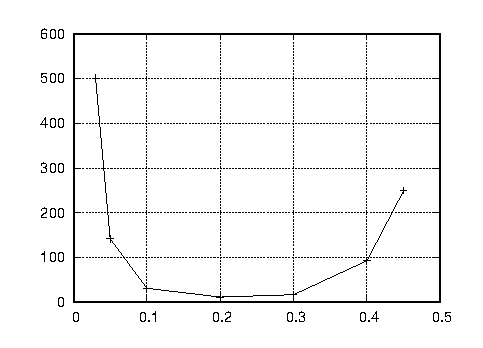
\includegraphics[width=0.5\hsize]{fig/modPerceptron.eps}
 \end{center}
 \caption{modPerceptron、収束までの反復回数}
 \label{fig:modPerceptron}
\end{figure}


\section{}
教科書の「HokkaidoTowns\_xy\@.dat」の各カラムがx y座標の座標値を表すとします。
このデータの重みベクトルによるボロノイ分割が、
y軸を境界とする2分割になりました。
この重みベクトルはどのようなものになるか例を使って説明しなさい。

\subsection{【回答】}
図\ref{fig:problem04}に例を示す。黒塗りの点が重みベクトルを示す。
白抜きの点は、各市町村である。中央の実線が$y$軸であり、
2つの重みベクトルの垂直二等分線になる。
すなわち、重みベクトルは、$y$軸に関して線対称になる。

\begin{figure}[tbp]
 \begin{center}
  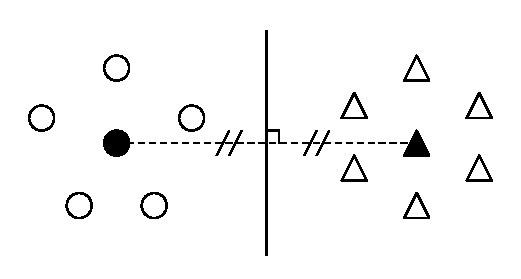
\includegraphics[width=0.5\hsize]{fig/problem04.eps}
 \end{center}
 \caption{課題4の例}
 \label{fig:problem04}
\end{figure}

\section{}
赤と青の2つの箱があり、
赤の箱にはりんごが2個とオレンジが6個、
青の箱にはりんごが3個とオレンジが1個入っているとする。
箱の1つをランダムに選び、果物をランダムに1個取り出す。
その際、赤の箱を40\%、青の箱を60\%選び、
箱の中の果物は別け隔てなく同じ確からしさで選ぶ。
この時、オレンジを選び出したとして、
それが青い箱から取り出されたものである確率はいくらか?
導出過程も含めて書きなさい。

\subsection{【回答】}

青い箱を選ぶ事象を$B$、オレンジを選ぶ事象を$O$とすると、
求める量は$P(B|O)$である。ベイズの定理より、
\begin{equation}
\label{p04sol}
P(B|O)=\frac{P(B)P(O|B)}{P(O)}
\end{equation}
題意より
\begin{equation}
P(B) = \frac{3}{5}, P(B^C)=\frac{2}{5}, P(O|B)=\frac{1}{4}, P(O|B^C)=\frac{3}{4}
\end{equation}
である。右肩の$C$は余事象を表す。例えば、$B^C$は赤い箱を選ぶ事象である。
これらを式(\ref{p04sol})に代入して、
\begin{equation}
(\textrm{式(\ref{p04sol})の分子})=\frac{3}{5}\times\frac{1}{4}=\frac{3}{20}
\end{equation}
\begin{eqnarray}
(\textrm{式(\ref{p04sol})の分母})&=&P(O) \\
&=& P(O,B)+P(O,B^C) \\
&=& P(B)P(O|B)+P(B^C)P(O|B^C) \\
&=& \frac{3}{5}\times\frac{1}{4}+\frac{2}{5}\times\frac{3}{4} \\
&=& \frac{3}{20}+\frac{6}{20} \\
&=& \frac{9}{20}
\end{eqnarray}
したがって、答えは
\begin{equation}
\frac{3}{20}\times\frac{20}{9} = \frac{1}{3}
\end{equation}
となる。

\section{}
教科書の表5\.2「フルーツのブレンド割合」の値は、
壷を選んだときに各フルーツが取り出される条件付確率を表しています。
今、各壷が選ばれる確率がすべて等しいとします。
この時、下記のフルーツポンチがあるとき、
それぞれの壷が選ばれたという「対数事後確率の大小関係を比較できる値」
を求め比較しなさい。

\subsection{【回答】}

\begin{equation}
\log P(C^k) + \sum_{m}x_m\log q_m^k
\end{equation}
を計算すればよい。ここで、$C^k$は壷$k$を選ぶ事象、$P(C^k)$はその確率、
$m$は果物の番号(たとえばマンゴーなら$m=1$、ナタデココなら$m=2$など)、
$x_m$は果物$m$の個数、$q_m^k$は壷$k$の中の果物$m$の割合である。
全ての$k$において$P(C^k)$は一定なので、これは無視してよく、結局
\begin{equation}
\sum_{m}x_m\log q_m^k
\end{equation}
を計算し、比較すればよい。\\
トロピカルの場合、
\begin{equation}
\log 0.5 + 2\log 0.1 + 3\log 0.03 + 5\log 0.04 \simeq -31.9
\end{equation}
クラシックの場合、
\begin{equation}
\log 0.05 + 2\log 0.1 + 3\log 0.1 + 5\log 0.1 \simeq -26.0
\end{equation}
山形の場合、
\begin{equation}
\log 0.03 + 2\log 0.1 + 3\log 0.15 + 5\log 0.4 \simeq -18.4
\end{equation}
山梨の場合、
\begin{equation}
\log 0.05 + 2\log 0.1 + 3\log 0.5 + 5\log 0.05 \simeq -24.7
\end{equation}
となる。従って、山形の壷である可能性が最も高い。

\section{}
フルーツポンチをgenPunchで生成し、
それをestParamで処理して、
モデルのパラメータを推定する実験をしなさい。
ボウルの数や果物の数を変えると、
推定結果の精度にどのような影響があるかについて考察しなさい。

\subsection{【回答】}
TBD

\begin{figure}[tbp]
 \begin{minipage}{0.5\hsize}
  \begin{center}
   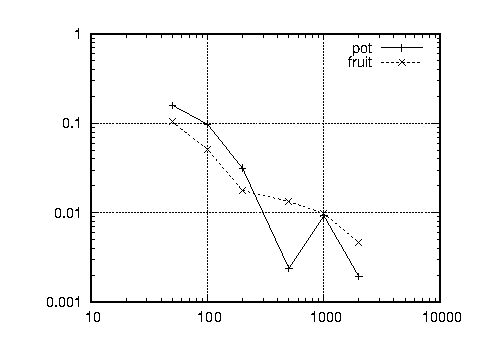
\includegraphics[width=\hsize]{fig/punch_pot.eps}
  \end{center}
  \caption{壷の数を振った時の誤差の変化}
  \label{fig:punch_pot}
 \end{minipage}
 \begin{minipage}{0.5\hsize}
  \begin{center}
   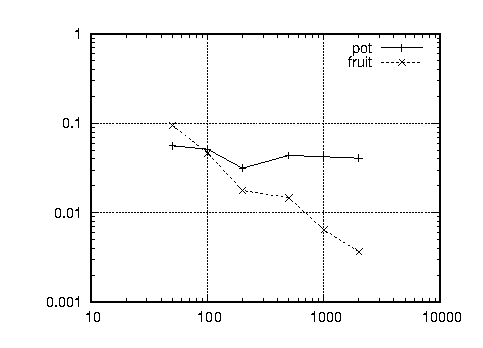
\includegraphics[width=\hsize]{fig/punch_fruit.eps}
  \end{center}
  \caption{果物数を振った時の誤差の変化}
  \label{fig:punch_fruit}
 \end{minipage}
\end{figure}

\end{document}
